\documentclass[12pt]{article} % The document class with options

\usepackage[margin=1in]{geometry}
\usepackage[utf8]{inputenc} 
\geometry{a4paper}
\usepackage{newtxtext,newtxmath}
\usepackage[T1]{fontenc}
\usepackage{amsmath}
\usepackage{amsfonts}
\usepackage{microtype}
\usepackage{graphicx}

% chktex-file 3
% chktex-file 8
% chktex-file 10
% chktex-file 17
% chktex-file 18
% chktex-file 36
% chktex-file 44

\begin{document}
\setlength{\parskip}{1em} 
\setlength{\parindent}{0pt}
\newcommand{\vect}[1]{\mathbf{#1}}

\begin{titlepage}  % This starts a title page environment
    \centering    % Center everything on the page

    %--- Add space at the top of the page ---
    \vspace*{2cm}
    
    %--- Title ---
    \normalsize \textbf{MECH 570C Project Report} \\
    \vspace{0.5cm}  % Space between lines
    \normalsize\textbf{A Comprehensive Review of Hydroelasticity of Ships} \\
    \vspace{2cm}  % Space between the title and the author name
    
    %--- Author ---
    \normalsize by\\
    \vspace{1cm}
    \normalsize Jincong Li \\ 
    \vspace{1cm}
    \normalsize M.Eng, The University of British Columbia, 2024
    \vspace{11cm}  % Space between the author and the date
    
    %--- Date ---
    \normalsize \today

    \vfill  % Push the following content to the bottom of the page
    %--- Bottom part of the page ---
    © Jincong Li, 2024
\end{titlepage}
\tableofcontents
\newpage
\section{Abstract}
Hydroelasticity, or the flexible fluid-structure interaction (FFSI), is a critical area of study within maritime engineering, focusing on the dynamic interplay between fluid forces and the elastic responses of structures. This report delves into the hydroelastic phenomena experienced by ships and offshore structures, with an emphasis on the implications of these interactions for ship design, offshore engineering, and renewable energy applications. It primarily explores the complex loading from waves, including phenomena such as springing, whipping, and sloshing loads, which significantly impact the structural integrity and operational viability of maritime vessels. Through a comprehensive review of both traditional computational methods and innovative approaches like the coupling of Computational Fluid Dynamics (CFD) and Finite Element Analysis (FEA), as well as emerging techniques involving neural networks, this report aims to highlight advancements and identify gaps in the current understanding of ship hydroelasticity. The findings underscore the necessity of integrating advanced simulation methods to enhance predictive capabilities and ensure the safety and efficiency of maritime operations.
\section{Introduction}
By definition, hydroelasticity or flexible fluid-structure interaction (FFSI), specifically deals with the dynamic interaction 
between fluid forces and elastic structural responses. This involves studying how structures deform under fluid forces and how these deformations, in turn, affect the fluid flow around them.
In maritime contexts, it refers to the responses of ships and offshore structures to ocean waves. And the modelling work will be conducted mainly by CFD and FEA.

There are several key applications:
\begin{enumerate}
    \item In ship design, it's essential for ensuring that ships can withstand the complex loading from waves, including the study of fatigue life due to repeated wave impacts.
    And also includes studying phenomena such as springing and whipping, which are high-frequency vibrations induced by waves, which will be our focus later.
    
    \item In offshore engineering, it facilitates the development of oil platforms and other marine structures that must withstand certain oceanic conditions, just as what we have seen in the course material.
    
    \item For renewable energy, it is crucial for designing durable floating structures such as wind turbines and tidal (taidal) generators.
\end{enumerate}

\newpage
\section{Motivation}
A paramount illustration of why hydroelasticity is essential involves the study of ultra large container ships as shown in figure 1 below. 
These vessels typically exhibit smaller block coefficients and substantial bow flares, attributes that increase their 
susceptibility to wave-induced loads, which will be reviewed in the next section. To clarify, the block coefficient is a dimensional ratio comparing the actual 
volumetric displacement of a ship to the volumetric displacement of a rectangular block defined by the ship’s length, 
breadth, and draft. A lower block coefficient indicates a more streamlined hull, enhancing hydrodynamic efficiency by 
reducing resistance, which in turn increases speed and fuel efficiency. And the bow, which is the front portion of the ship, 
features a design element known as the bow flare. This design refers to the outward and upward curvature of the ship's bow above the waterline. 
The primary function of the bow flare is to deflect water away from the ship's deck as it navigates through waves. An effectively designed bow flare 
can significantly mitigate the impact of waves against the ship, commonly referred to as slamming. However, ultra large container 
ships often have a more aggressive bow flare than typical vessels, which may also introduce certain challenges. These 
challenges include potential stability issues and increased sensitivity to specific wave conditions, necessitating careful consideration in hydroelastic analyzes and ship design.
\begin{figure}[ht]
    \centering
    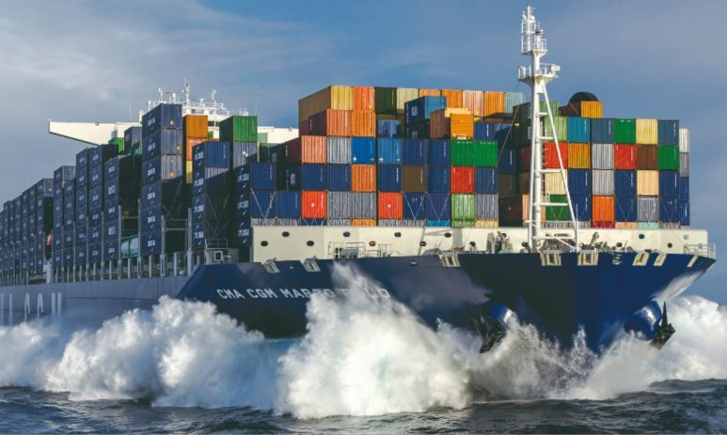
\includegraphics[width=1\textwidth]{ULCS.png}
    \caption{Example Ultra Large Container Ship}
\end{figure}

Smaller block coefficients and substantial bow flare is evident in the design of the S175 model ship, a standard used in both experimental and numerical simulations shown in figure 2. 
Its transversal body plan demonstrates a smooth contour extending from bow to stern, designed to optimize streamlining. 
Consequently, while such designs confer advantages in speed and fuel consumption, they also render the ship more vulnerable 
to the impacts of wave-induced loads due to their refined hydrodynamic profiles. This sensitivity underscores the critical 
importance of hydroelastic studies in ensuring the structural integrity and operational viability of these large vessels under dynamic ocean conditions.
\begin{figure}[ht]
    \centering
    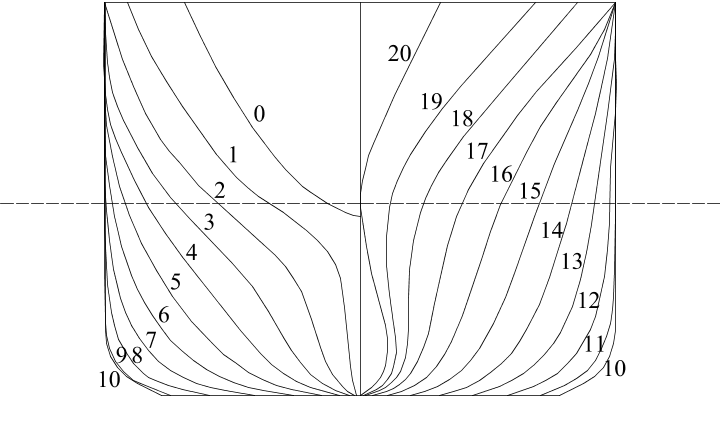
\includegraphics[width=1\textwidth]{S175_transverse.png}
    \caption{Transversal body plan of the S175 hull\cite{1}}
\end{figure}

% The Bow is the front part of the ship and the bow flare refers to the outward and upward curvature of the ship's bow above the waterline. It helps to deflect water away from the ship’s deck as it cuts through waves. A well-designed bow flare could make the ship feels less slamming against waves, however, those ultra large container ships might have a larger bow flare than usual, which might cause some problems.
\clearpage
\section{Wave Induced Load}

The wave induced load could be classified into three categories. The first category, termed "springing," is defined by significant elastic deformation in the hull that 
resonate both in-plane and out-of-plane with the frequencies of encountered waves. A distinct category of induced loads 
known as "whipping" arises from nonlinear, impulsive wave actions that are often associated with interactions at the bow flare, 
the bottom, or the stern of the ship. This phenomenon is prominently observed in various types of vessels including passenger ships, 
container ships, liquid natural gas carriers, and warships. Another critical type of load is referred to as "sloshing loads." 
These are highly impulsive forces exerted on the cargo containment systems of gas ships, which have the potential to cause 
localized structural damage to the walls of the tanks.

Understanding induced wave loads phenomenons are essential to study "Hydroelasticity of Ships", and the outcome of this subject is to what is the consequences of 
those loads. Here are several findings 
published by the International Ships and Offshore Structure Congress (ISSC) and the International Towing Tank Conference (ITTC) 
technical committees\cite{1}: 
\begin{enumerate}
    \item High-frequency components of the vertical bending moment due to whipping 
    can be as large as the wave-frequency component; 
    \item The total bending moment can exceed traditional rule design values of 
    slender vessels; 
    \item Both springing and whipping loads are relevant for the assessment of fatigue limit states; 
    \item Ultimate limit states are primarily influenced by whipping responses; 
    \item Sloshing loads may lead to local damages of cargo containment 
    systems. 
\end{enumerate}

\section{Sea Accidents}
In this section, some real sea accidents of ultra large container ships are reviewed to understand the consequences of wave induced load. The first example shown in figure 3 involved a United Kingdom-flagged vessel 
that sustained a hull breach under conditions of rough seas and significant slamming. A detailed analysis by the UK Marine Accident Investigation Branch (MAIB) revealed that the vessel's 
structural failure was primarily due to insufficient reinforcement in the engine room's framing. The inquiry noted that during the incident, wave-induced loads on the ship were intensified by 
approximately 30\%, possibly as a result of whipping effects.

Another case is that of the MOL Comfort, which suffered a catastrophic structural failure, resulting in the midship section fracturing. 
The vessel ultimately split into two and sank. The subsequent accident investigation suggested that the structural integrity of the ship was 
compromised by wave loads that exceeded its design limits. It was consequently recommended that future regulatory standards should incorporate 
considerations for lateral and whipping loads in the assessment of maritime structural strength.
\begin{figure}[ht]
    \centering
    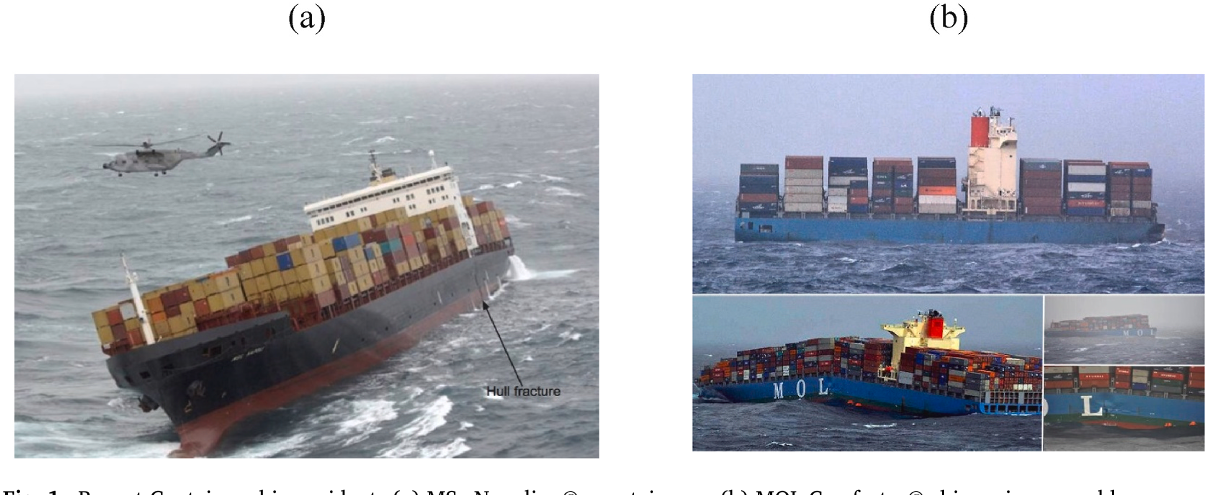
\includegraphics[width=1\textwidth]{SA.png}
    \caption{Example Sea Accidents}
\end{figure}
After seeing those accidents and investigating a lot, some researchers suggests: (i) the excess of the vertical bending moment that is larger than the ultimate 
strength capacity can be redistributed to the inertia and hydrostatic restoring moments associated with plastic hull girder deformations; (ii) the 
plastic deformation develops to a much smaller degree due to whipping moment than due to normal wave-induced loads possibly because of the limited 
time during which the plastic deformations grow following whipping. In a follow-up study it is shown that the plastic deformation can accumulate 
gradually under a series of extreme whipping moments that exceed the ultimate strength, and the rate of accumulation can grow after large accumulation 
of the plastic deformation. Thus, some advice in designing the ships are brought up, for example, by a leading-edge organization called DNV, they introduced partial safety factor of 0.9 reducing 
the effectiveness of whipping during collapse\cite{1}.

\section{Numerical Approach}
From 1979, plenty of work has been done on both 2D and 3D hydroelasticity theory within the framework of potential flow theory\cite{2}\cite{3}, as some researchers pointed out: 
flow field during slamming and green water event is highly nonlinear and cannot be accurately represented using potential flow methods\cite{4}.
Therefore, the computational fluid dynamics techniques became interesting. However, applying CFD itself is not enough, although global motions and external loadings could be obtained by CFD simulation, the hull sectional loads, e.g. 
vertical bending moment and shear force, used for wave loads analysis cannot be directly obtained from the CFD simulation. Moreover, the majority of current 
CFD applications are limited to simulating fluid flow around a rigid body. Thus, it is essential to couple CFD with FEA. More work has been done in fully coupled approach\cite{5} or some kind of special treatment\cite{6}.

One significant finding is that, all these works suggest that the high frequency hydroelastic vibrations cannot be directly simulated in the one-way coupling method since the structural 
deformation of hull is not considered in the CFD simulation. Thus, the two-way coupling is more accurate to reproduce the hydroelastic effects of flexible ship in waves\cite{4}.

\section{CFD \& FEA Coupling}
As stated in the last section, there are two method to couple CFD and FEA: one-way coupling and two-way coupling, as shown in figure 4. 
In the one-way interaction model, the hull is treated as rigid within the fluid domain. Here, the fluid dynamics simulation applies wave loads to the structure, 
but does not account for any deformations of the structure in the fluid dynamics calculations. This approach is typically adopted when the impact of structural 
deformation on hull loading and fluid dynamics is considered negligible, offering the benefit of significantly reduced computational costs. However, even under 
this framework, a two-way coupling analysis may be employed to assess the structural response in addition to rigid body motions, although it does not take into 
account the effect of structural deformations on the fluid dynamics. Notably, the added mass effect on structural vibrations is omitted in this one-way coupling scenario.

Conversely, in the two-way interaction model, there is a significant interplay between the fluid and the structure, meaning that structural deformations influence 
and are influenced by the fluid dynamics. This method allows for the incorporation of the added mass and its real-time variations resulting from changes in the 
wetted surface area throughout the period of wave interaction. The two-way interaction approach thus provides a comprehensive assessment of the dynamic interactions 
between the structure and the fluid, capturing the nuances of their mutual influence.
\begin{figure}[ht]
    \centering
    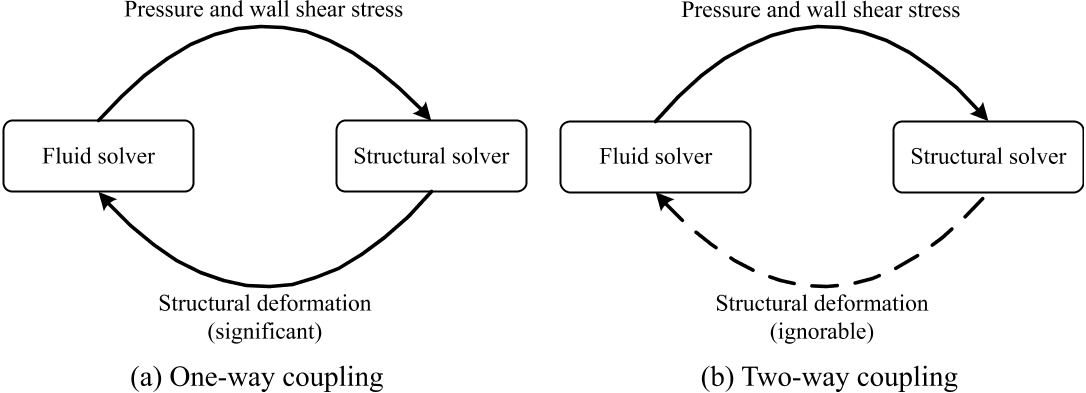
\includegraphics[width=1\textwidth]{OT.png}
    \caption{One-way Coupling vs. Two-way Coupling}
\end{figure}

\subsection{Two-way Coupling}
Two-way coupling can be further classified into explicit and implicit couplings, the schemes are shown in figure 5. For weaker fluid-structure interaction (FSI) scenarios, 
such as the static deformation of a flexible hydrofoil in uniform flow, where after several transient interactions the system approaches a 
steady-state with minimal structural velocities, an explicit coupling method is typically favored. This method facilitates calculating the 
transient processes before achieving steady-state equilibrium, with information exchanges occurring once per time step.

Conversely, in cases where there is a significant time-dependent interdependence between the fluid and structural responses, and minor 
changes in one solver promptly affect the other, an implicit coupling method is advisable. Figure 15 illustrates the frameworks for both 
explicit and implicit coupling between computational fluid dynamics (CFD) and finite element analysis (FEA) solvers.

A partitioned algorithm is employed to implement the two-way coupling, with information sequentially exchanged and iteratively solved 
between the CFD and FEA solvers. In the implicit coupling model, exchanges of fluid loads and structural deformations occur three times 
per time step, a frequency that is crucial to ensure the accuracy, convergence, and computational efficiency of the simulations. 
Each time step includes twelve iterations to manage both the global rigid body movements and the hull’s flexural motions, which are computed within ABAQUS.
\begin{figure}[ht]
    \centering
    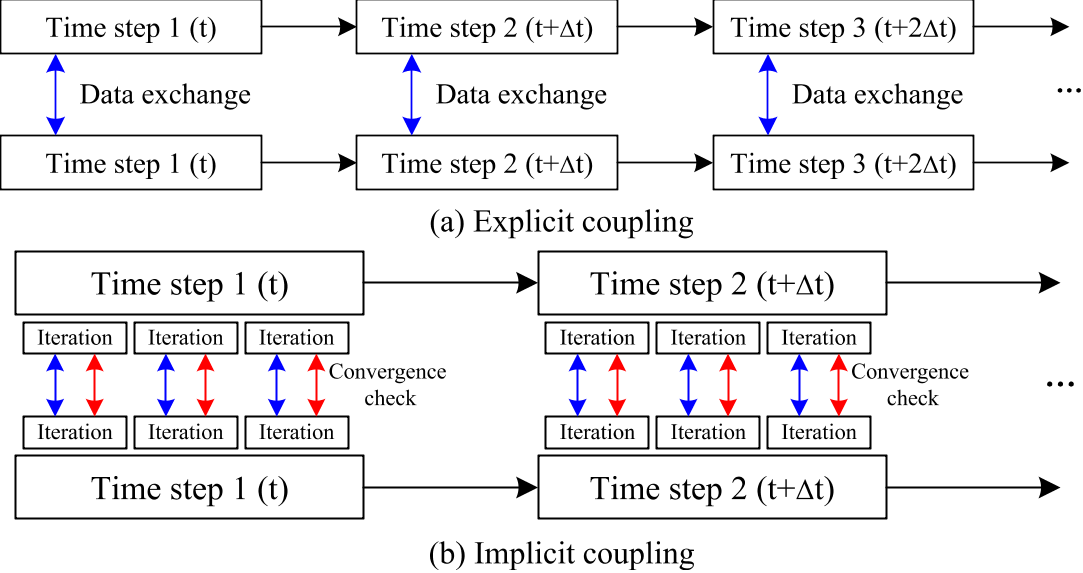
\includegraphics[width=1\textwidth]{Loop.png}
    \caption{ Two-way Coupling Scheme\cite{4}}
\end{figure}
\section{Simulation Results}
This section will review the simulation result shown in\cite{4} and their conclusion.
The paper\cite{4} systematically analyzes ship motions, vertical accelerations, and wave loads, including springing and whipping responses, under various wave conditions. A significant highlight is the reproduction of high-order hull girder vertical vibrations, such as 12th order harmonic springing and 4-node whipping responses.
The method applied in\cite{4} demonstrated high reliability in simulating complex nonlinear hydroelastic responses in waves. Additionally, complex flow phenomena like slamming and green water on deck were successfully captured, showcasing the advanced capabilities of the CFD–FEA co-simulation method.
The simulation data were captured and analyzed in both time domain and frequency domain (figure 6\&7), and then validated against available experimental data and other numerical methods, confirming the accuracy of the simulation approach.


\begin{figure}[ht]
    \centering
    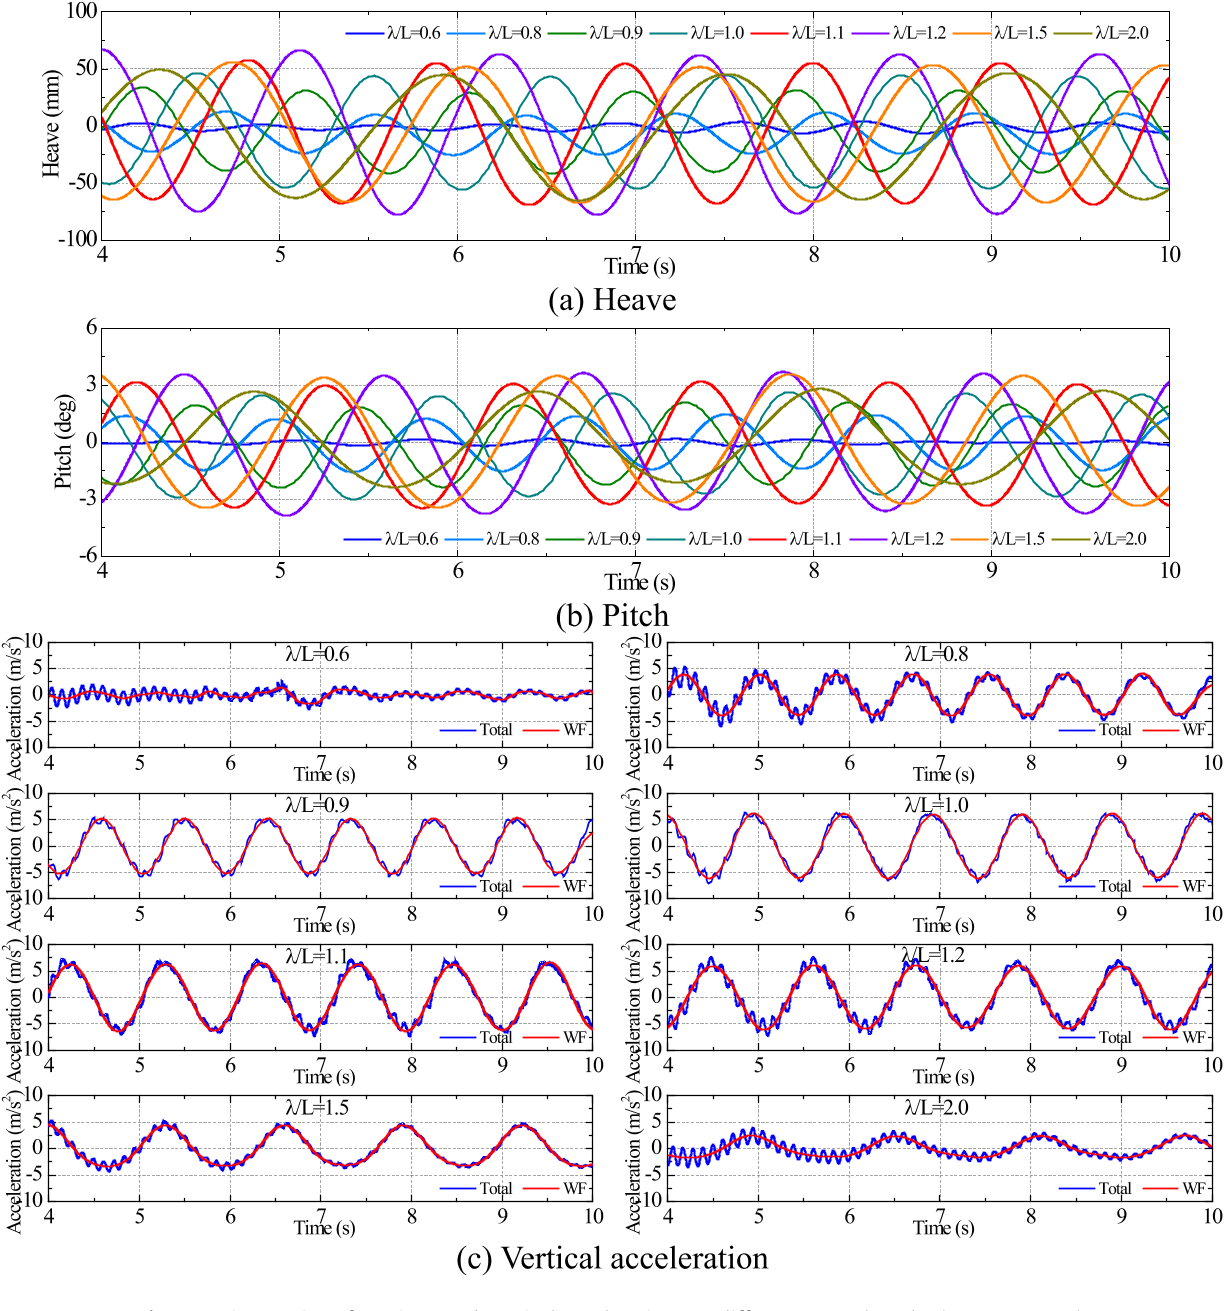
\includegraphics[width=1\textwidth]{HPV.png}
    \caption{Data in Time Domain\cite{4}}
\end{figure}
\begin{figure}[ht]
    \centering
    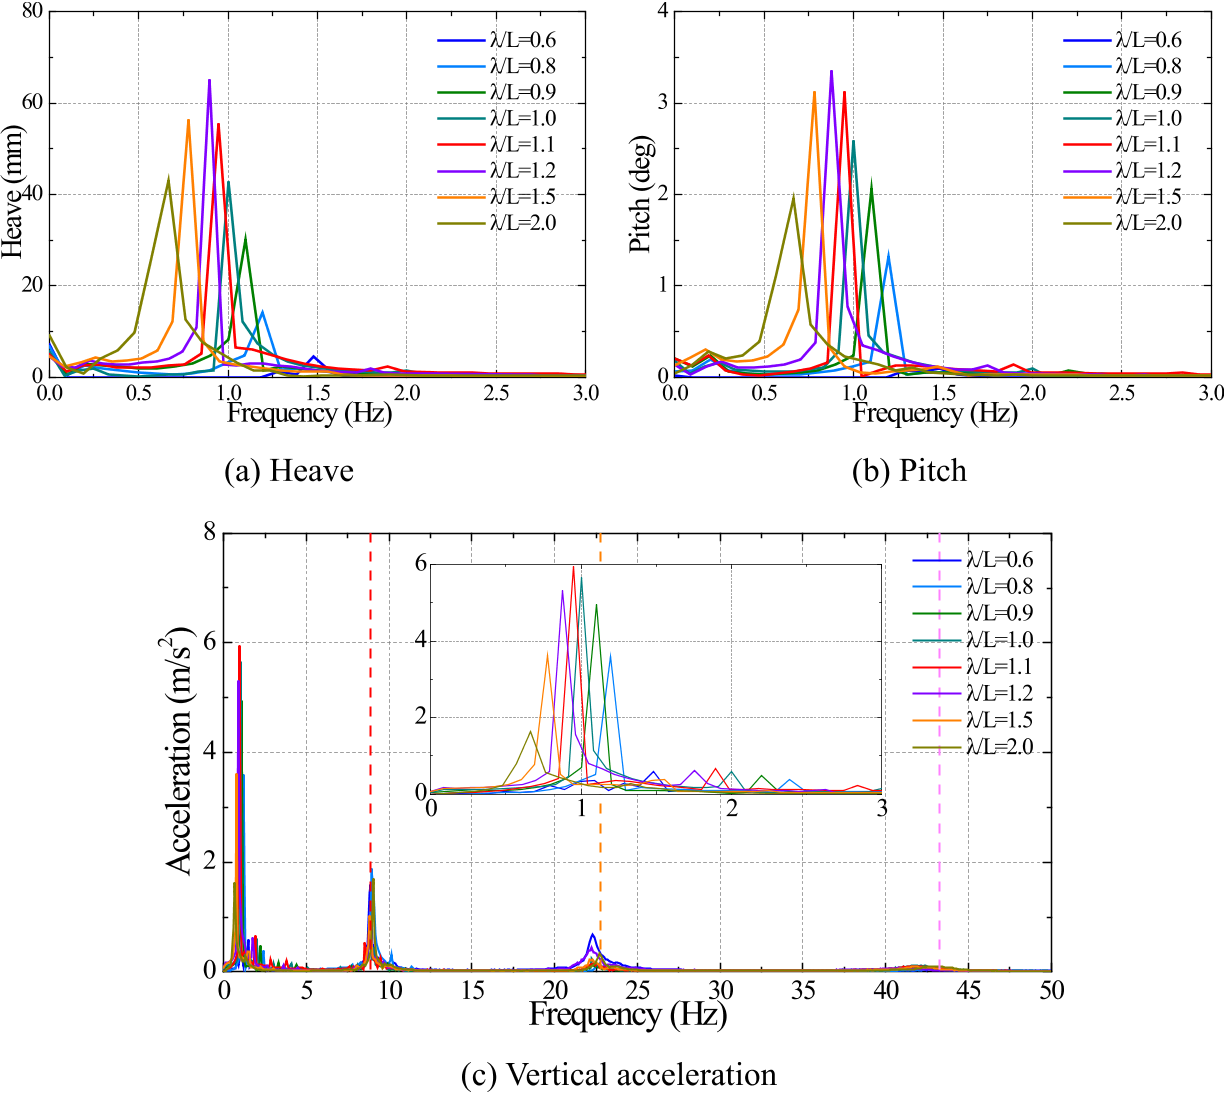
\includegraphics[width=1\textwidth]{FD.png}
    \caption{Data in Frequency Domain\cite{4}}
\end{figure}

\clearpage
\section{Neural Network}
\cite{7} demostrated a LSTM-based model which is trained on a comprehensive dataset that includes motion data and vertical bending moment history under various sea states, achieved through numerical simulations. And the author pointed out that 
the LSTM-based encoder-decoder model effectively captures and predicts global whipping responses, offering a promising tool for enhancing maritime safety and highlighted the model's potential applicability in real-world scenarios, emphasizing its effectiveness in generalizing across different sea states.
\begin{figure}[ht]
    \centering
    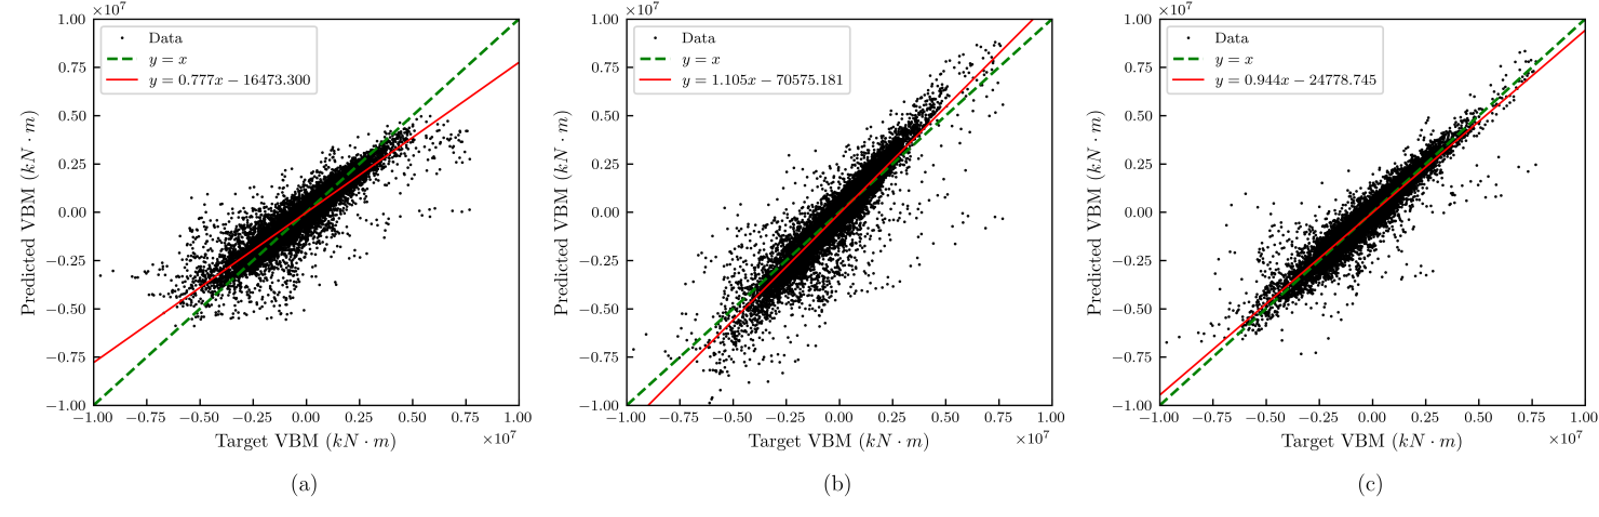
\includegraphics[width=1\textwidth]{RNN.png}
    \caption{THE COMPARISON BETWEEN THE TARGET AND PREDICTED RESULTS\cite{7}}
\end{figure}

\clearpage
\section{Conclusion}
The study of hydroelasticity, particularly in the context of ship design and maritime operations, is of paramount importance due to the critical nature of the interactions between 
oceanic forces and structural responses. This work systematically reviewed the key aspects of hydroelastic phenomena affecting ships, including the detailed analysis of 
wave-induced loads such as springing, whipping, and sloshing, which pose significant threats to ship stability and integrity. Through the examination of various computational 
techniques, from traditional CFD and FEA simulations to advanced LSTM-based neural networks, it is evident that modern engineering approaches offer significant improvements 
in predicting and mitigating the effects of these complex interactions. The integration of two-way coupling methods in simulation practices represents a particularly promising 
advancement, enabling more accurate representations of the real-time interactions between fluid dynamics and structural responses. Moreover, the application of machine learning 
models like the LSTM encoder-decoder highlights the potential for further enhancing predictive accuracy and operational decision-making in unknown sea states. Overall, this 
report not only reinforces the understanding of hydroelastic impacts on maritime structures but also sets the stage for future research directions that could lead to more 
robust design strategies and safer maritime operations. Future studies should focus on refining these computational models and exploring their applications in real-world 
scenarios to fully harness the potential of hydroelastic analysis in improving maritime safety and design efficiency.
\begin{thebibliography}{99}

    \bibitem{1}
    Hirdaris, S., Parunov, J., Qui, W., Iijima, K., Wang, X., Wang, S., … Guedes Soares, C. (2023). Review of the uncertainties associated to hull girder hydroelastic response and wave load predictions. Marine Structures, 103383. 

    \bibitem{2}
    Bakica, A., Malenica, Š., \& Vladimir, N. (2020). Hydro-structure coupling of CFD and FEM - Quasi-static approach. Ocean Engineering, 108118. https://doi.org/10.1016/j.oceaneng.2020.108118
    
    \bibitem{3}
    Hirdaris, S. E., \& Temarel, P. (2009). Hydroelasticity of ships: Recent advances and future trends. Proceedings of the Institution of Mechanical Engineers, Part M: Journal of Engineering for the Maritime Environment, 223(3), 305–330. https://doi.org/10.1243/14750902jeme160
    
    \bibitem{4}
    Jiao, J., Huang, S., \& Guedes Soares, C. (2021). Viscous fluid–flexible structure interaction analysis on ship springing and whipping responses in regular waves. Journal of Fluids and Structures, 106, 103354. https://doi.org/10.1016/j.jfluidstructs.2021.103354
    
    \bibitem{5} 
    Paik, K.-J., \& Carrica, P. M. (2014). Fluid–structure interaction for an elastic structure interacting with free surface in a rolling tank. Ocean Engineering, 84, 201–212. https://doi.org/10.1016/j.oceaneng.2014.04.016
    
    \bibitem{6} 
    Bakica, A., Malenica, Š., \& Vladimir, N. (2020). Hydro-structure coupling of CFD and FEM - Quasi-static approach. Ocean Engineering, 217, 108118. https://doi.org/10.1016/j.oceaneng.2020.108118
    
    \bibitem{7}
    Liu, R., Li, H., Muk, C., Ong, O., \& Zou, J. (n.d.). PREDICTION OF GLOBAL WHIPPING RESPONSES ON A LARGE CRUISE SHIP UNDER UNKNOWN SEA STATES USING AN LSTM BASED ENCODER-DECODER MODEL.
\end{thebibliography}
\end{document}